\section{Resources Allocation}\label{sec:resAlloc}
In this section the resource allocation for the tasks related to \emph{PowerEnJoy} project will be presented; it uses the high level tasks shown in the \hyperref[sec:schedule]{schedule section} to describe which tasks will be assign to each of the team members.

\subsection{Notes for the charts}
\begin{itemize}
	\item The duration of the first task of each diagram represents the number of working days in the interval of dates defined by the starting date of the first actual task assigned to the resource, and the ending date of the last one; in between this interval there may be days in which the resource has no assigned tasks. This was done to leave some elasticity to the project in order to avoid further delays in the project development.
	\item The \emph{Resource Names} column contains the names of the team members who will collaborate with the resource in order to accomplish a given task. If this field is empty, it means that the resource will work on that task on his own.
\end{itemize}

\begin{figure}[h]
	\centering
	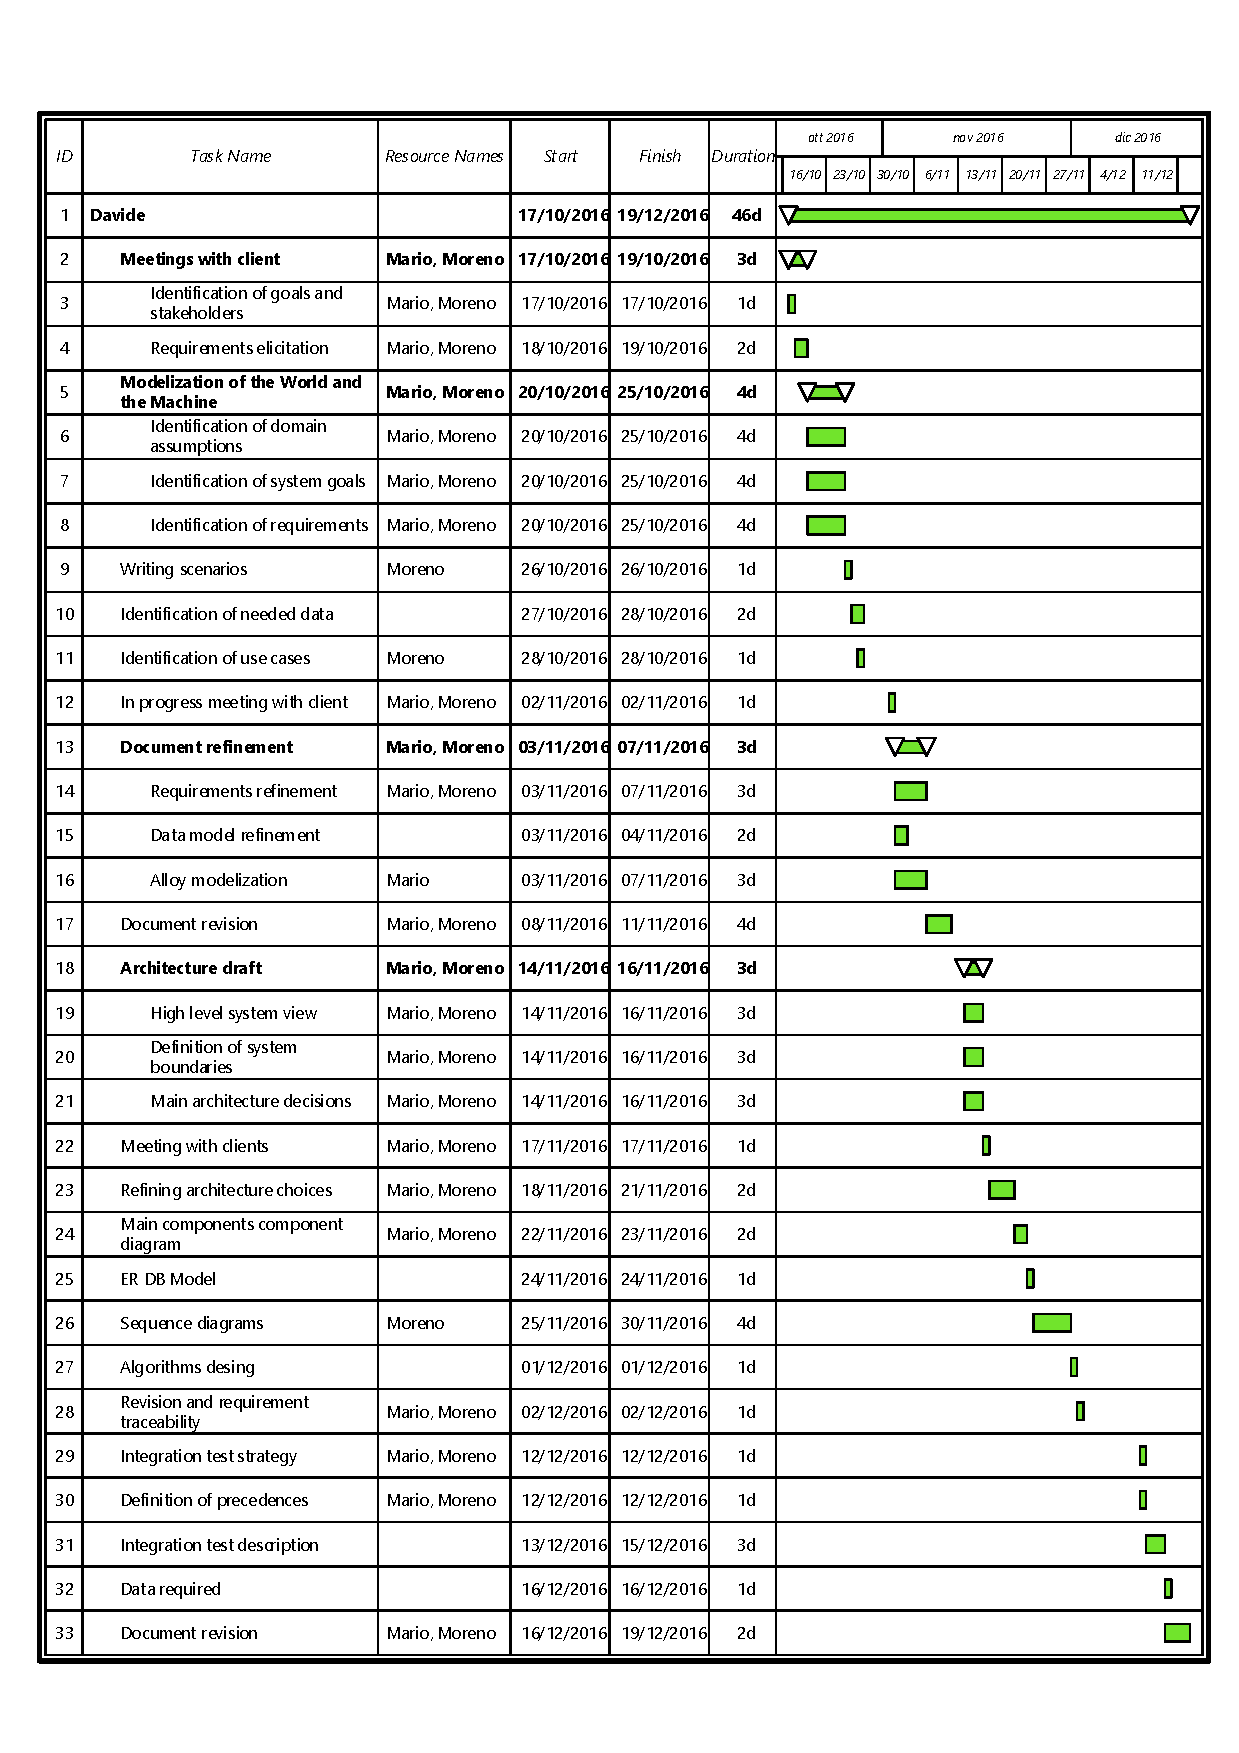
\includegraphics[width=\linewidth]{DavideGantt}	\caption{
		\label{fig:davideGantt} 
		Davide Piantella tasks Gantt chart
	}
	
\end{figure}\begin{figure}[h]
	\centering
	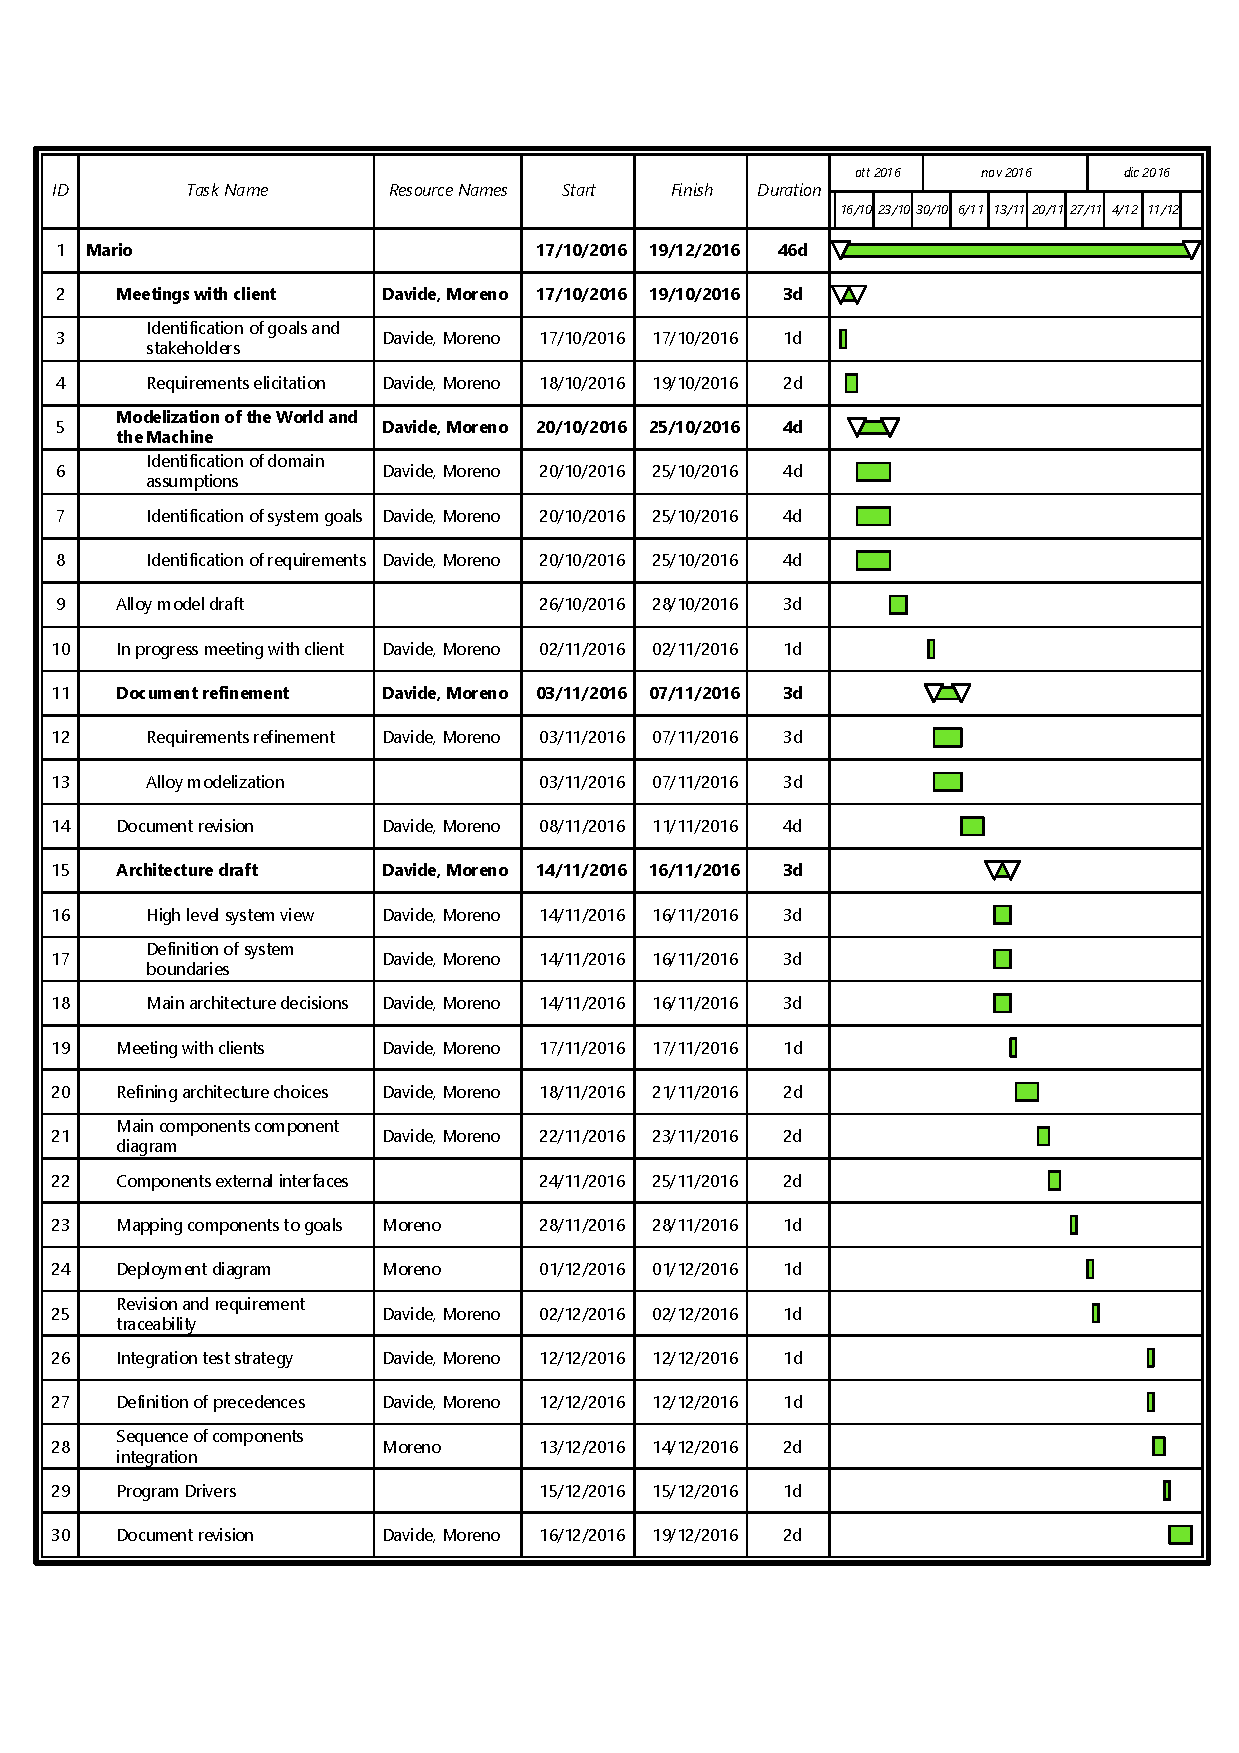
\includegraphics[width=\linewidth]{MarioGantt}	\caption{
		\label{fig:marioGantt} 
		Mario Scrocca tasks Gantt chart
	}
	
\end{figure}\begin{figure}[h]
	\centering
	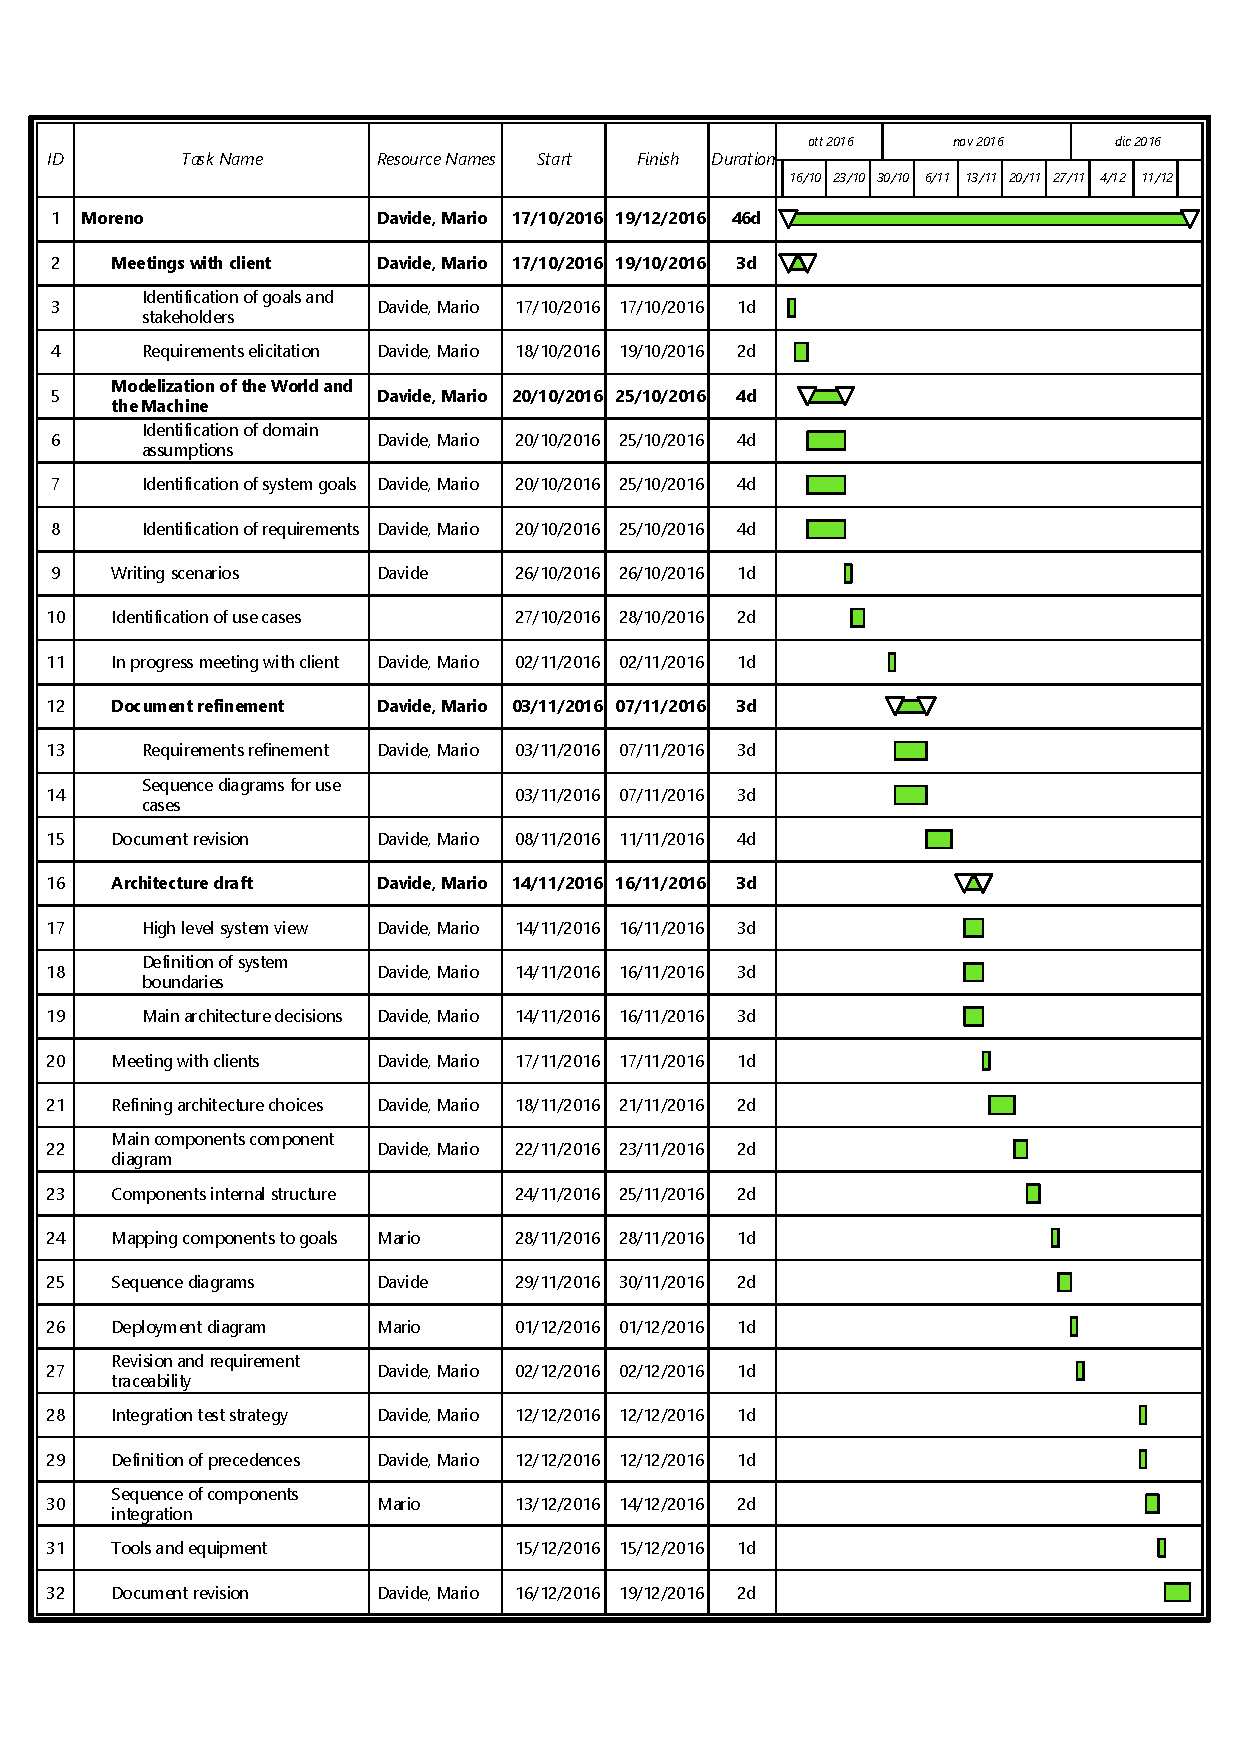
\includegraphics[width=\linewidth]{MorenoGantt}	\caption{
		\label{fig:morenoGantt} 
		Moreno Raimondo Vendra tasks Gantt chart
	}
\end{figure}